\chapter{Mathematical problem definition}
\label{chap3:title}
\nomenclature{SCA}{Single Connector Attachment}

This chapter opens the model from the mathematical point of view and defines the problem that should be solved in the paper. In the beginning of the chapter we consider the parameters that describe how many commands should be sent for the complete erasure of all amount of disks and in which order. Later we model the dynamic load balancing system, which could help with improving the speed, and, finally, we pose the optimization problem. After that we try to estimate what kind of limitations exist from theoretical and technical sides. This part of the chapter gives an idea what we should expect during practical tests of the erasure. Moreover, it helps to understand what parameters we should take into consideration more during searching the solution for our problem.

\newpage
\section{Communication model between SCSI controller and SCSI disks}
Currently the time costs a lot that is why it is important to make programs as fast as possible. Because of that optimization problem is one of the most significant ones. In general it is the problem of finding the best solution from the set of all feasible solutions. It is often done with different algorithms, which analyse the solutions during variable changing. In our case the optimization problem is based on time optimization. That means that the time will be optimized by several variables which can be changed.

Lets consider the model presenting on the picture \ref{fig:conn_model}, which shows how SCSI controller is connected to the disks and CPU (Central processing unit). This picture can be divided to 5 parts: CPU, where Blancco software is running, bus \emph{a} - from CPU through motherboard to the SCSI controller, SCSI controller \emph{b}, buses \emph{c} - from SCSI controller to the disks \emph{d}. Let consider that the SCSI controller is connected to $N$ disks.

\begin{figure}[h]
\begin{center}
  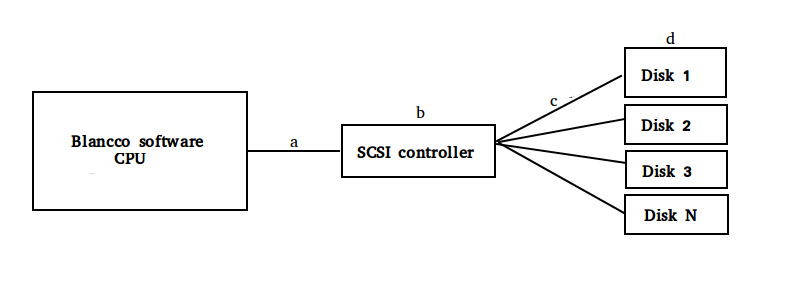
\includegraphics[width=0.95\textwidth]{conn_model}
\end{center}
  \caption{Communication model of SCSI controller}
  \label{fig:conn_model}
\end{figure}

This Figure presents how SCSI controller is connected in our case.  

All the time people want to do everything as fast as possible, but of course there are limitations in different places. The same situation is in this model - each part has the limitation of the speed. Moreover, there are also limitations for the memory.


Lets consider the Figure \ref{fig:conn_model} more detailed. In this model CPU part will be skipped, because there are so powerful computers in current time that it should not be taken into consideration. The main idea of Blancco software is to write the data to the disks. Lets discuss what \emph{data} means in this context. On the Figure \ref{fig:conn_model} there are $N$ disks and each of them has its own capacity $d_i$, where $i=\overline{1,N}$ shows the number of the disk. Capacity $d_i$ is calculated in megabytes. Each disk $i$ should get the amount of data, which is at least equal to the capacity of the disk. Moreover, we maybe need to send the commands for setting the connection with the disk. 


We discussed in the section \ref{subsec:write_comm} that Blancco software uses two different versions of write command. Each of these commands has its own capacity. Let define these capacities in a mathematical way. The capacity of the WRITE command is $c_1$, the capacity of the WRITE SAME command is $c_2$ and the capacity of other commands is $c_3$. In these context other commands means the commands for identification the device and setting the connection. All these three variables $c_1$, $c_2$, $c_3$ are constant and are defined by Blancco software. Hence for replacing all data on $N$ disks it should be sent $F$ MB from SCSI controller \emph{b} to the disks \emph{d} through the buses \emph{c}. Let $F$ be called as \emph{complete erasure}, is it is calculated by the following formula:
\begin{equation}
\label{eq:comp_erasure}
	F = \sum_{i=1}^{N}F_i,
\end{equation}
where $F_i$ is the amount of megabytes, that should be sent to the disk $i$, which is calculated as
\begin{equation}
	F_i = c_1 m_{i1} + c_2 m_{i2} + c_3 m_{i3},
\end{equation}
where $m_{ik}$ is the number of times that command $c_k$ should be sent, where $k=\overline{1,3}$. Furthermore, complete erasure $F$ should fulfil the following condition:
\begin{equation}
\label{eq:write_cond}
	c_1 c_2 = 0, \forall F_i, i=\overline{1,N}.
\end{equation}
This condition means that only 1 command $c_1$ or $c_2$ can write to each disk. Thus the software can not erase the same disk with both commands $c_1$ and $c_2$. That means that only software decides which command is better to use and dynamic load balancing system should apply the strategy how to apply it more efficiently.


For clear vision and comprehension it is convenient to present the set of $F_i$ as a matrix $F_m$:
\begin{equation}
	F_m =
	\begin{pmatrix}
		F_1\\ \vdots\\ F_N 
	\end{pmatrix}
	=
	\begin{pmatrix}
		c_1 m_{11} & c_2 m_{12} & c_3 m_{13} \\
		\ldots & \ldots & \ldots \\
		c_1 m_{N1} & c_2 m_{N2} & c_3 m_{N3} \\
	\end{pmatrix},
\end{equation}
where $F_m$ is the matrix with dimension $N\times3$.

The capacity of each disk $i$ should be less than amount of data, which is sent for writing. That means that the following condition should be fulfilled:
\begin{equation}
	d_i < F_i, i=\overline{1,N}.
\end{equation}
But this condition is true only for the WRITE command $c_1$, because the WRITE SAME command $c_2$ sends the same buffer several times, which means that we do not need to send this buffer all the time. Thus, for the WRITE SAME command $c_2$ we have another condition:
\begin{equation}
	d_i > F_i, i=\overline{1,N}.
\end{equation}

The main aim of the research is to find the way how to send the data faster to the disks. Of course, that it depends on all the devices that are in the model, on the strategy how the software sends the commands and also on the parameters of the command that we use for erasure. Let define the variable $S_{max}$ for maximum speed and it is obvious that this variable is constant. According to the formula \ref{eq:comp_erasure} and maximum speed $S_{max}$ it is possible to calculate the minimum time $T_{min}$ for realization complete erasure $F$ by the following formula:
\begin{equation}
\label{eq:time_min}
	T_{min} = \sum_{i=1}^{N}t_i 
			= \frac{\sum_{i=1}^{N}F_i}{S_{max}}
			= F/S_{max},
\end{equation}
where $t_i$ is the time for sending $F_i$ MB to $i$ disk with the maximum speed $S_{max}$. 



\section{Mathematical problem definition}
Let consider that in the same model there is dynamic load balancing system and it calculates the application state $m=F/s$ times, where $F$ is the amount of megabytes to complete the application task and $s$ is the step. In this context step $s$ means the amount of commands and $m$ means how many times the dynamic load balancing system should apply another input data for the next step.

There is matrix $H=\{h_{ij}\}$, where $i=\overline{1,N}$ is the disk number, $j=\overline{1,m}$ is the step number of the dynamic load balancing system and $h_{ij}$ is the number of commands, which is sent to the $i$ disk at $j$ step. That means that for complete erasure $F$ we need the following amount of commands:
\begin{equation}
\label{eq:load_balancing_matrix}
	\sum_{i=1}^{N}\sum_{j=1}^{m}h_{ij} = \sum_{i=1}^{N}\sum_{k=1}^{3}m_{ik}.
\end{equation}
As an example of matrix $H$ it is convenient to consider 4 disks, which can be erased by 100 commands with the condition that we can not send more than 100 commands per step. Thus the matrix $H$ can be presented as 
\begin{equation}
	H_1 =
	\begin{pmatrix}
		100 & 0 & 0 & 0 \\
		0 & 100 & 0 & 0 \\
		0 & 0 & 100 & 0 \\
		0 & 0 & 0 & 100 \\
	\end{pmatrix}
\end{equation}
or a bit more complicate:
\begin{equation}
	H_2 =
	\begin{pmatrix}
		50 & 10 & 20 & 20 \\
		20 & 50 & 10 & 20 \\
		20 & 20 & 50 & 10 \\
		10 & 20 & 20 & 50 \\
	\end{pmatrix}.
\end{equation}
Matrix $H_1$ and $H_2$ are practical examples of the matrix $H$. The first matrix shows the trivial strategy - to send as many commands as the program can to fulfil the condition during each step. Matrix $H_2$ shows that it could be done in a different way and we can divide the whole amount of commands and send it separately. The strategy should be applied by some dynamic load balancing algorithm and the aim of the research is to find out what is the optimal matrix $H_{opt}$ and could load balancing help in this case or not.

Also there is matrix $Q=q_{ij}$, where $q_{ij}$ is the order number in the queue for sending commands to $i$ disk at $j$ step. In this case it is possible to show to which disk the program should send the command first. The dimension of $Q$ is the same as dimension of $H$: 
\begin{equation}
	\dim(Q) = \dim(H) = N \times m,
\end{equation}
where $N$ is the number of disks and $m$ is the number of steps in the load balancing system. Of course, that if we apply the parallel strategy matrixes $H$ and $Q$ do not make any sense, because we will not know how many commands are sent to which device. 

For mathematical problem definition it is convenient to introduce the functional of time. Let the \emph{functional of time} be defined as the functional 
\begin{equation}
	T=\sum_{j=1}^{m}t_j,
\end{equation}
where $t_j$ is the time for sending $\sum_{i=1}^{N}h_{ij}$ commands at $j$ step of dynamical load balancing process.

The main idea of the optimization problem is to minimize the functional of time $T$
\begin{equation}
\label{opt_problem}
	\min_{F,H,Q,s}T.
\end{equation}
According the formula \ref{eq:time_min} current minimization problem can be rewritten as
\begin{equation}
	T \xrightarrow[F,H,Q,s]{} T_{min}.
\end{equation}
That means that the application of dynamic load balancing algorithm should make the program faster and the value of $T$ should come close to the minimum time $T_{min}$. The algorithm should use $F$, $H$, $Q$, $s$ as parameters for making the program faster. As it was mentioned usage parallel strategy removes some of these parameters and the amount of megabytes $F$, which we need to send to erase all $N$ disks, starts to be the most important value. But complete erasure $F$ also hides some interesting parameters such as amount of sending commands and buffer size of the command, which will play quite important role in the following paper.

\section{Technical limitations}
Every device has its own technical limitations. For example, a car has a limitation for the speed, capacity of petrol tank, maximum engine power and so on. Discussing the SCSI controllers every device has special characteristics, which we can compare with characteristics of the car.

Let introduce some parameters, which can influence on the communication between controller and disk. 
In this paper the word SCSI is used a lot, but there was no clear explanation what is it. As it is written in the beginning of the paper SCSI is Small Computer System Interface. The main word in this abbreviation is interface, which shows \emph{how} the devices can be connected with each other. Lets again consider the Figure \ref{fig:conn_model} and the situation that we write some data from CPU to the disk. Controller \emph{b} has 2 interfaces, because it is connected to the CPU and disks \emph{d}. Let call bus \emph{a} as \emph{input} interface and buses \emph{c} as \emph{output} interface. For the disks \emph{d} there is only input interface, that is why it is possible to skip the word \emph{input} and use only interface. So, if there is a sentence, which includes "the controller has SCSI interface", that means that the controller has the possibility to connect SCSI disks and the output interface is SCSI. Moreover, because controller has 2 connections there is also input interface, which can be, for example, different modifications of PCI (Peripheral component interconnect) such as PCI-X, PCI64, PCI Express or some others. In general words if there is a discussion about SCSI interface it means only the buses \emph{c}.

Moreover, SCSI is also a data protocol, which shows what commands can be sent through buses \emph{c}. Depends on the previous content SCSI interface connection has different technical limitations. There are several SCSI interfaces such as SCSI-1, Fast-Wide SCSI, Ultra2 SCSI, Ultra-320 SCSI and some others, but in this research Ultra-320 SCSI interface will be considered more, because the testing device is supported that interface. Nowadays there is interface with faster bandwidth - 640 MB/s - but it did not get popular, because it supports maximum 2 devices per cable.

Ultra320 SCSI \cite{ultra320} is the seventh generation of SCSI I/O (Input/Output) technology. The dominant feature is that the speed is increased to 320 megabyte per second (MB/s). In Ultra320 SCSI devices all support packetized protocol and may support Quick Arbitration and Selection (QAS). Expander communications techniques have also been defined. In general Ultra320 shows that only buses \emph{c} from the Figure \ref{fig:conn_model} have this speed and not disks \emph{d}, and of course, not controller \emph{b}. In the ideal situation to get the maximum speed of the device communication we should fulfil the following condition:
\begin{equation}
	S_a > S_b > S_c > S_d.
\end{equation}
Otherwise there is a question, how controller is going to manage several disks if it has the same speed.
Currently there are different PCI buses, which can have the maximum bandwidth up to 4 GB/s. Moreover, there are also some possibilities to increase the performance of PCI \cite{increase_pci}. But even it is not the limit, because there are also some other buses, such as QPI (QuickPath Interconnect) and HyperTransport with different modification, which can easily have the bandwidth around 25 GB/s. By now the maximum bandwidth has HyperTransport 3.1 with value 51,20 GB/s. Of course, that bus depends on the frequency quite a lot. HyperTransport 3.1 has the maximum frequency 3,2 GHz. Depends on the data content and the number of the disks the data for the transport through bus \emph{a} can increase, but the numbers show that it seems that it is not a problem, but still it is better to keep this fact in mind.

%Other features are included: paced data transfer, a free running clock, a training pattern at the beginning of a transfer series, skew compensation, driver pre-compensation and/or optional receiver Adjustable Active Filter (AAF). 


All SCSI devices are always backward compatible, which means that when newer SCSI devices are attached to a system with devices from a previous generation, the newer devices will fall back to the maximum operating speed of the older generation when they are talking. When not talking to older devices, the newer devices operate at their normal speeds. That means that if one of SCSI drives from the Figure \ref{fig:conn_model} works on Ultra160 interface, the controller, which supports Ultra320, will talk to the disk using Ultra160 interface.

Most of the time in the hardware if the device or cable can be connected to some place that means that it will work. The same situation is with SCSI interfaces, but for some generations connectors are the same. For the interfaces Ultra2 Wide, Ultra3, Ultra320 and Ultra640 the connectors can be 68-pin and 80 pin which belongs to the connection type SCA/SCA-2 (Single Connector Attachment). The examples of the connectors are presented on the Figure \ref{fig:SCA_conn}.
\begin{figure}[h]
\begin{center}
	\label{fig:SCA_conn}
  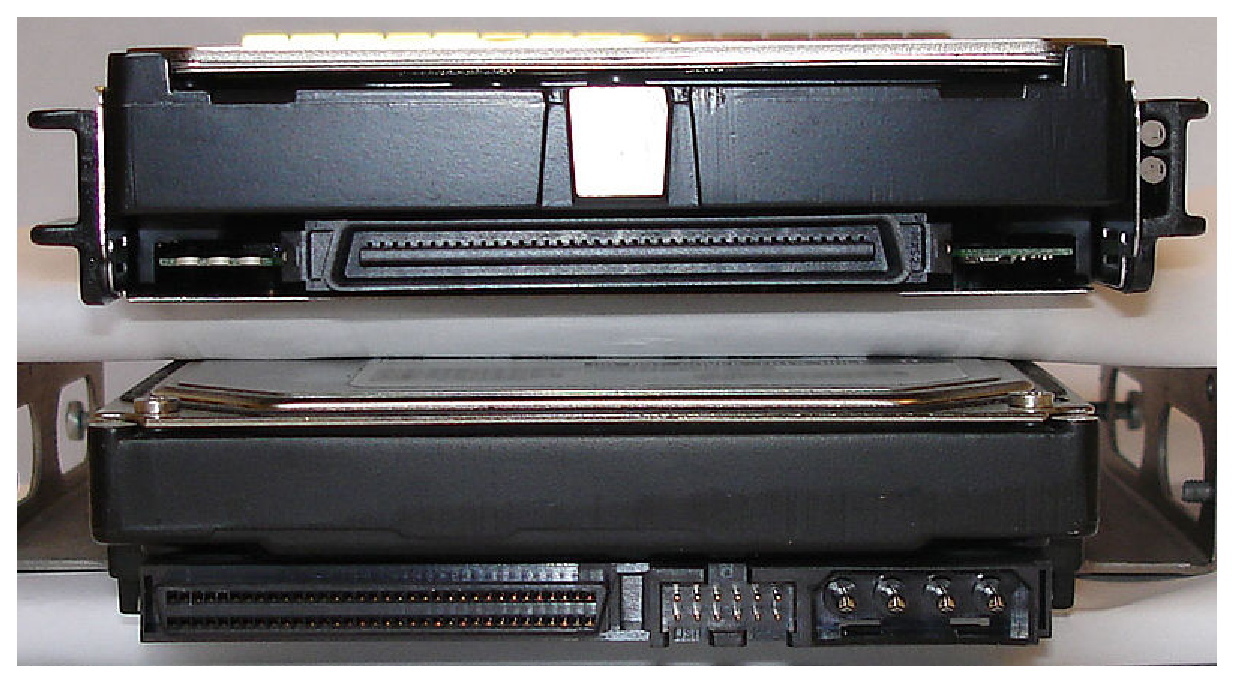
\includegraphics[width=0.95\textwidth]{SCA_conn}
\end{center}
  \caption{68-pin and 80-pin SCA connectors}
  \label{fig:SCA_conn}
\end{figure}


Mostly the discussion about technical limitations contained the information about the buses \emph{a} and \emph{c}, but what about controller and disks? Let start from the disks. In this chapter it was already introduced that each disk $i$ has capacity $d_i$, speed $S_d$ and special interface. But there are some other parameters, which could be also important. It is \emph{cache}, \emph{spindle speed}, average \emph{seek time} for reading and writing, connector type and dimension. The last parameter is not very interesting, because we assume that there is enough space.

In general cache is used in many situations, for example, in operation systems, in controllers, in disks and some other places. Cache is the part of memory, which has very fast speed access \cite{intro_scsi_perform}. For the disks it means that cache is stored before the physical hard disk platter, which gives the possibility to get the data much faster. Currently disks can have cache with capacity from 8 to 64 MB. Of course, that big cache gives higher performance for the disk. Moreover there are different cache algorithms such as LRU (Least Recently Used), MRU (Most Recently Used), LFU (Least-Frequently Used), Direct-mapped cache and some others \cite{cache_alg}, \cite{cache_strategies}. The aim of every cache algorithm is to manage the data in the cache and show, which data block to delete and which one to keep. Depends on the disk it can be applied different cache algorithms, which could give the advantage or disadvantage in the current problem. Also, depends on the number of the disks maybe load balancing system should find some tricky steps through disk cache, which can make the process faster.

Another important characteristic of disk is spindle speed, which shows the frequency of rotation. This value is measured in revolutions per minute (RPM). The value of spindle speed shows how many full rotations were completed in one minute around a fixed axis. Usually for ATA disks spindle speed can be 5400 or 7200 rpm (90 or 120 Hz) and in this case SCSI disks win, because their spindle speed can be 10,000 or 15,000 rpm (160 or 250 Hz). This value is constant and is set by manufacture. So, there is no reason to try make it higher, the only possibility is to take the disk with higher spindle speed.

Both of described parameters cache and spindle speed are influenced on the seek time of the disk. Seek time means the time, which needs for the head of the disc to move to the right position. It is clear that this time can be only average, because in different situations there are different values of cache, spindle speed and data task. In general there are two values of seek time - one for reading operations and another for writing, but usually it is only one value for both operations. Most of the time in the research it will be considered only as a writing seek time, but the value of seek time for the reading should not be thrown out. There are two seek measurements called track-to-track and full stroke. The track-to-track measurement is the time required to move from one track to an adjacent track. This is the shortest (fastest) possible seek time. In hard disk drives (HDD) this is typically between 0.2 and 0.8 ms. The full stroke measurement is the time required to move from the outermost track to the innermost track. This is the longest (slowest) possible seek time.

Lets consider the controller now and figure out what parameters this device has. First of all, it has the possibility to connect buses \emph{a} and \emph{c}, which was decided to call as input interface and output interface, which also follow the specific parameter, such as speed. In the literature it is also possible to see that input interface is called as host interface. Secondly, it is the amount of RAIDs, which is supported by this controller. There are also some more parameters, which are still important, such as cache, cache function or algorithm, maximum amount of physical disks, maximum amount of logical disks. We discussed what does cache mean and controllers cache has more power in comparison with disk cache. Currently cache of the controllers can have values up to 512 MB. Moreover, some controllers have even their own cache algorithms, which make it stronger. But this fact is obvious, because the controller should have enough power to communicate with all connected disks.

There is one parameter, which should be marked out. It is the bandwidth of the controller, which definitely influences on the performance of the device. But most of the time in the parameters of the controller it is possible to find only the bandwidth of the input and output interfaces. It is like this, because currently the controllers are so powerful, that they can manage all the data, which comes to the device. That means that the speed of the controller is not the bottleneck and is not very important in our case.

\section{Theoretical estimations}
\label{sec:theory_est}

Lets model the real situation and try to estimate how long time does it take to write some data to the disk. Let consider that there is a Compaq SCSI disk BD01864552 with the following parameters: 
\begin{itemize}
	\setlength{\itemsep}{-2mm}
	\item Capacity: 18.2 GB
	\item Spindle speed: 10,000 RPM
	\item Interface: Ultra3 SCSI
	\item Seek time: 3 ms
\end{itemize}
From these parameters mostly we will focus on the interface, which has a speed 160 MB/s. That means that the speed of the bus c is equal to 320 MB/s. Basically all data on disks are divided to the sectors. Most of the time the size of the sector is 512 bytes, but in some cases this value can be different. In this research we consider that the sector size has 512 bytes value. We will focus on the parameters of the commands and the disks because the controller should not be a bottleneck, but we still need to think that there are some limitations also in the controller.

\paragraph{WRITE SAME command}
Let consider the WRITE SAME 10 command, which comes from the CPU \cite{scsi3_bc}. This command has 32 bits for the LBA (Logical block addressing) and 16 bits for the Number of Logical Blocks. The main huge advantage of that command is that we can send the same buffer to several logical blocks only with one command. It gives us a possibility to write much more data than we really send by the command.

We can calculate the maximum amount of data that we can write with one WRITE SAME 10 command to the disk:
\begin{equation}
	\frac{2^{16}*512}{1024^2} = 32 MB.
\end{equation}
Let consider that the model \ref{eq:comp_erasure} consists of 1 disk and we do not need any other commands except WRITE SAME one. That means that in condition \ref{eq:write_cond} parameter $c_2$ will be equal to 0. We also assume that we do not need any special commands for the communication and $c_3$ is equal to 0. It gives a possibility to calculate complete erasure $F$ as a multiplication of command $c_1$ and amount of commands $m_{11}$. Because we know the capacity of the disk we could compute the number of commands $m_{11}$ that we need to send for erasure 18.2 GB disk.
\begin{equation}
	m_{11} =\frac{F_1}{c_1} = \frac{18.2*1024}{32} = \frac{18636.8MB}{32MB} = 582.4.
\end{equation}
For performance of real erasure the data should be divided for filling the last part of the disk, because we could not send 0.4 command. The main aim of the research is testing the erasure time that is why we will not take this little part into consideration and will use the approximate value of 582.

The size of WRITE SAME 10 command is 10 bytes. Including the buffer, which is 512, we get that one whole command is 522 B.
So, to erase one 18.2 GB disk we need to send the following amount of data:
\begin{equation}
	F_1 = (10 + 512)*582 = 303804 B = 304 kB.
\end{equation}
That means that for complete erasure of one disk we need to send only 304 kB. Another command WRITE 10 does not have so huge advantage, but lets compare these two commands, because in some cases WRITE SAME 10 command does not work.

% So, the most important question is the writing time to the whole disk. It can be calculated, because bus speed and the amount of % buffer for one write command are known:
% This can be wrong (we divide apple by apelsin)
% \begin{equation}
%	T = F_1/S_c = 18432/160 = 115.2 sec = 1.92 min.
% \end{equation}

\paragraph{WRITE command}
Let consider another pass through command WRITE 10 \cite{scsi3_bc}. The structure of this command is completely the same in comparison with WRITE SAME 10 command, but some parameters have different values. For example, WRITE SAME 10 command has operation code 0x41 and WRITE 10 command has 0x2A. The main difference of these 2 commands is that with WRITE 10 command we need to send whole buffer all the time. The buffer length is calculated by the following Formula:
\begin{equation}
	Buffer~length = Sector~size * Tranfer~length.
\end{equation}
In our situation the disks have constantly sector size 512 and this value depends only on the disk. But buffer length can be varied by transfer length, which can have a value up to 65536. That means that if we decide to set the maximum transfer length we could send 32 MB with one WRITE 10 command. In comparison with WRITE SAME 10 command, which has 512 B buffer, our buffer can increase to 512*65536, which is quite big value if we consider that the controller connect to several disks. Usually, in Linux driver of the controller there is a value of maximum buffer, which is 4096*512 in our case. It can be optimal for some amount of disks, but it should be checked, because this is one of the parameters that we can influence.

If a lot of data go with one command through the controller it can make the erasure process slower because the cache of the controller will be full of messages, waiting in the queue. We should influence on the erasure speed by this parameter and find the optimal value during testing. By now this value is set to 256, which means that we send 128 kB at once. We can calculate how many commands we need to erase one 18.2 GB disk by WRITE 10 command with 128 KB buffer:
\begin{equation}
	m_{11}=\frac{F_{1}}{c_{2}}=\frac{18.2GB}{128kB}=\frac{18636.8MB}{0.125MB}=149094.4
\end{equation}
The derived value is 256 times bigger than the amount of commands that we need to send for erasure by WRITE SAME. It is obvious, because the current value of buffer length is 256 bigger. In the chapter  \ref{chap4:title} we will see the results of erasure testing with different transfer lengths.














